\begin{filecontents}{leer.eps}
%!PS-Adobe-2.0 EPSF-2.0
%%CreationDate: Mon Jul 13 16:51:17 1992
%%DocumentFonts: (atend)
%%Pages: 0 1
%%BoundingBox: 72 31 601 342
%%EndComments

gsave
72 31 moveto
72 342 lineto
601 342 lineto
601 31 lineto
72 31 lineto
showpage
grestore
%%Trailer
%%DocumentFonts: Helvetica
\end{filecontents}
%
\documentclass[epj]{svjour}
% Remove option referee for final version
%
% Remove any % below to load the required packages
%\usepackage{latexsym}
%\usepackage{graphics}
\usepackage{graphicx}
\usepackage{epstopdf}
\usepackage[utf8]{inputenc}
% etc
%
\begin{document}
%
\title{Network analysis of metabolic subsystems}
%\subtitle{Do you have a subtitle?\\ If so, write it here}
\author{Rok Novosel\thanks{\email{rn0450@student.uni-lj.si}} \and Matija
  Čufar\thanks{\email{matijacufar@gmail.com}}
% \thanks is optional - remove next line if not needed
%\thanks{\emph{Present address:} Insert the address here if needed}%
}                     % Do not remove
%
\institute{Faculty of Computer and Information Science}
%
%\date{Received: date / Revised version: date}
%
\abstract{Subsystems are parts of a metabolism that perform different important
  tasks in a cell. In this article, we explore these subsystems from a network
  science point of view. We attempt to find ways of detecting subsystems in a
  metabolic network using community detection algorithms.  We use the Louvain
  modularity optimization algorithm and the Clauset-Newman-Moore algorithms as a
  baseline against which we compare the effectiveness of other algorithms. As a
  comparison, we use the Girvan-Newman algorithm and a motif-based community
  detection approach. We present the results on a metabolic network of the
  Chinese hamster ovary cell, a mammalian cell that is commonly used in
  biomedical research and in biotechnology.}

% tole gre v abstract
%\PACS{
%      {PACS-key}{discribing text of that key}   \and
%      {PACS-key}{discribing text of that key}
%     } % end of PACS codes

\maketitle

\section{Introduction}
\label{sec:intro}

Since the turn of the century, life sciences have been evolving
rapidly. Advances in data acquisition, storage and analysis technology have
allowed scientist to gather immense amounts of data and build complex models
from it~\cite{modsys}. These complicated models have brought people of various
backgrounds, such as physics, mathematics and computer science into the field
of biology.

One such field is network science, which
is often used to analyze different kinds of networks that appear in the various
subfields of modern biology, including ecology~\cite{proulx2005network}, systems
biology~\cite{barabasi2004network} and neuroscience~\cite{sporns2014contributions}.

Metabolic networks~\cite{jeong2000large} are used to model the meta-bolisms of
various organisms. They are usually represented with a bipartite graph composed
of two types of vertices: reactions and chemicals produced and consumed by the
reactions. The edges in such a network connect chemicals to
reactions. Furthermore, the edges are directed indicating whether the chemical
was produced or consumed. A third kind of vertex can be added to represent
enzymes that catalyze the reaction, but do not directly partake in
it. Other commonly used representations are simplified representations, where
one of the types of vertices is omitted~\cite{newman2010networks}.

In this article, we analyze the subsystems in a metabolic network of the Chinese
hamster ovary cell. We explore different methods of detecting the subsystems and
compare their structures, focusing on the Girvan-Newman
method~\cite{girvan2002community} and an approach based on network
motifs~\cite{benson2016higher}. We expect these algorithms to outperform other
commoly used algorithms such as Louvain optimization or the Clauset-Newman-Moore
algorithm.

\section{Related works}
\label{sec:related}
% benson2016higher - motifs
% jeong2000large - scale free
% holme2003subnetwork

In~\cite{jeong2000large}, Jeong et. al offer a general overview of the
organization and structure of metabolic networks. The authors compare the
metabolic networks of 43 different organisms and find that metabolic networks
belong to the class of scale-free networks. Moreover, they find that the network
diameter is consistent across all of the analyzed networks, irrespective of the
number of substrates found in the given species.

In~\cite{holme2003subnetwork}, Holme et. al present a method to decompose
metabolic networks into subnetworks based on the global network structure. They
use a modified Girvan-Newman algorithm~\cite{girvan2002community} to construct a
hierarchical clustering tree. They argue that instead of looking at a particular
partitioning of a network, we should look at the hierarchical clustering tree as
whole, since well-defined subnetworks appear at different heights.

A framework for clustering networks based on higher order structures
(e.g. motifs) is introduced in~\cite{benson2016higher}. The authors of the
article present an algorithm that performs community detection by using three
node motifs. It works by cutting the network into communities in a way that
minimizes the ratio of the number of motifs cut to the number of nodes in
instances of the motif.

\section{Methods}
\label{sec:methods}

In this article, we analyse a metabolic network of the Chinese hamster
ovary (CHO) cell. The CHO cell is frequently used in biological and medical
research and in the production of biopharmaceuticals~\cite{chocons}.

We use a whole-cell metabolic network of the Chinese hamster ovary (CHO)
cell that was taken from the BiGG database~\cite{bigg,chocons}. The original
network contains 4,456 metabolites that take part in 6,663 reactions. The
reactions and metabolites are annotated with additional metadata, such as name,
subsystem, BiGG ID etc.

The network was simplified to a simple directed graph, where reactions are
represented with nodes. If one reaction produces a metabolite that is used by
another reaction, they are connected by an arc. This network has 6,663 nodes and
656,609 arcs. If we treat as an undirected network, it has 546,208 edges.

We use two commonly used network community detection algorithms, namely the
Louvain modularity optimization algorithm~\cite{blondel2008fast} and the
Clauset-Newman-Moore algorithm~\cite{clauset2004finding}, as the baseline and
compare them to motif-based clustering methods~\cite{benson2016higher}.

The motif-based clustering method, motif counting and the Clauset-Newman-Moore
algorithm were taken from the SNAP library~\cite{leskovec2016snap} and the
Louvain modularity optimization algorithm was taken from the Networkx Python
library~\cite{networkx}.

\section{Results}
\label{sec:results}

The network has a very large connected component of 6,036 nodes, while the other
components are very small, as they are composed of at most 4 nodes. The largest
connected component contains a strongly connected component of 5,307 nodes,
while the other nodes are isolated. These probably represent sources and sinks
of the metabolism.

The network appears to have a scale-free structure. Its in-degree, out-degree
and degree distributions are plotted in figure~\ref{fig:dist}. Some commonly
used network properties are presented in table~\ref{tab:metrics}.

\begin{table}
  \centering
  \begin{tabular}{l|l|l|l}
    $C_d$ & $C_u$ & $E_{90}$ & $\rho$ \\
    0.012 & 0.069 & 15 & 0.015
  \end{tabular}
  \caption{The directed and undirected clustering coefficients $C_d$ and
    $C_u$, effective diameter $E_{90}$ and the density $\rho$ of the network.}
  \label{tab:metrics}
\end{table}

First, we count the appearances of all 13 directed three-node motifs in the
network. The significances~\cite{milo2002network} of each motif are presented in
the second row of table~\ref{tab:motifs}. The significances were calculated by
comparing the motif occurances with 10 instances of Erdős-Rény random graphs of
the same size and density.

The normalized mutual information scores of the motif based clustering approach
are listed in the last row of table~\ref{tab:motifs}. We have calculated these
scores by comparing the algorithm's results and the actual subsystems listed in
the network annotation. The results are not the best, but still much better than
the Louvain and the Clauset-Newman-Moore method, listed in
table~\ref{tab:others}. We partly attribute the quality of the results to the
fact that most biological networks tend to be noisy.

\emph{NOTE: we plan on also using Infomap and the Girvan-Newman algorithms, but
  it seems like they will take a few more days to compute.}

\begin{figure}
  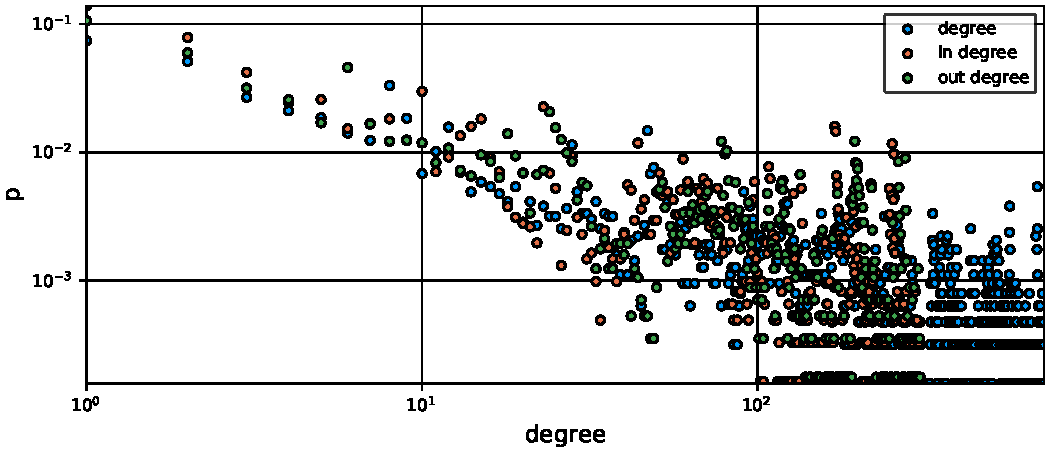
\includegraphics[width=0.45\textwidth]{../plots/degreesmall}
  \caption{The in-degree, out-degree and degree distributions of the network,
    plotted on a log-log scale.}
  \label{fig:dist}
\end{figure}

\begin{table*}[t!]
  \centering
  \begin{tabular}{l|lllllllllllll}
    \hline\noalign{\smallskip}
    &
    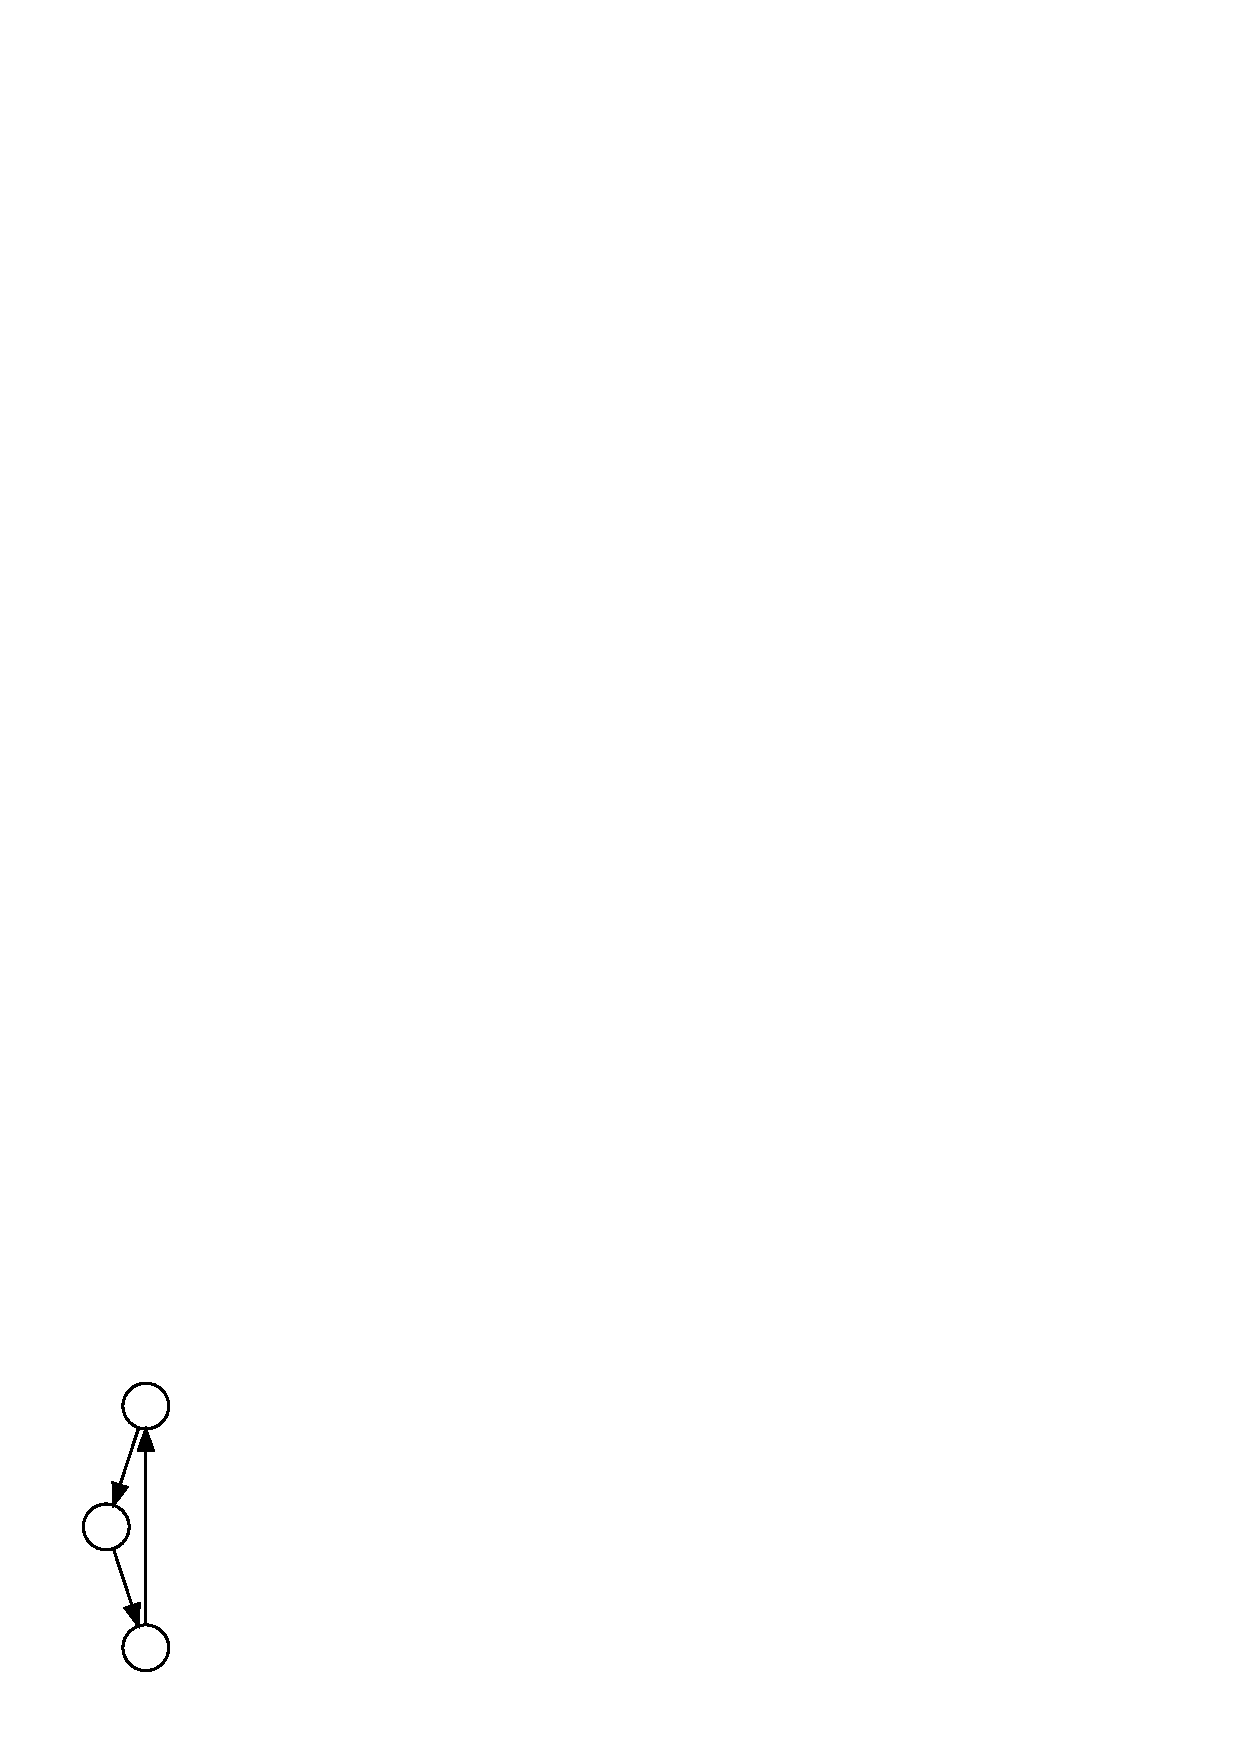
\includegraphics[height=0.03\textheight]{M1-plain} &
    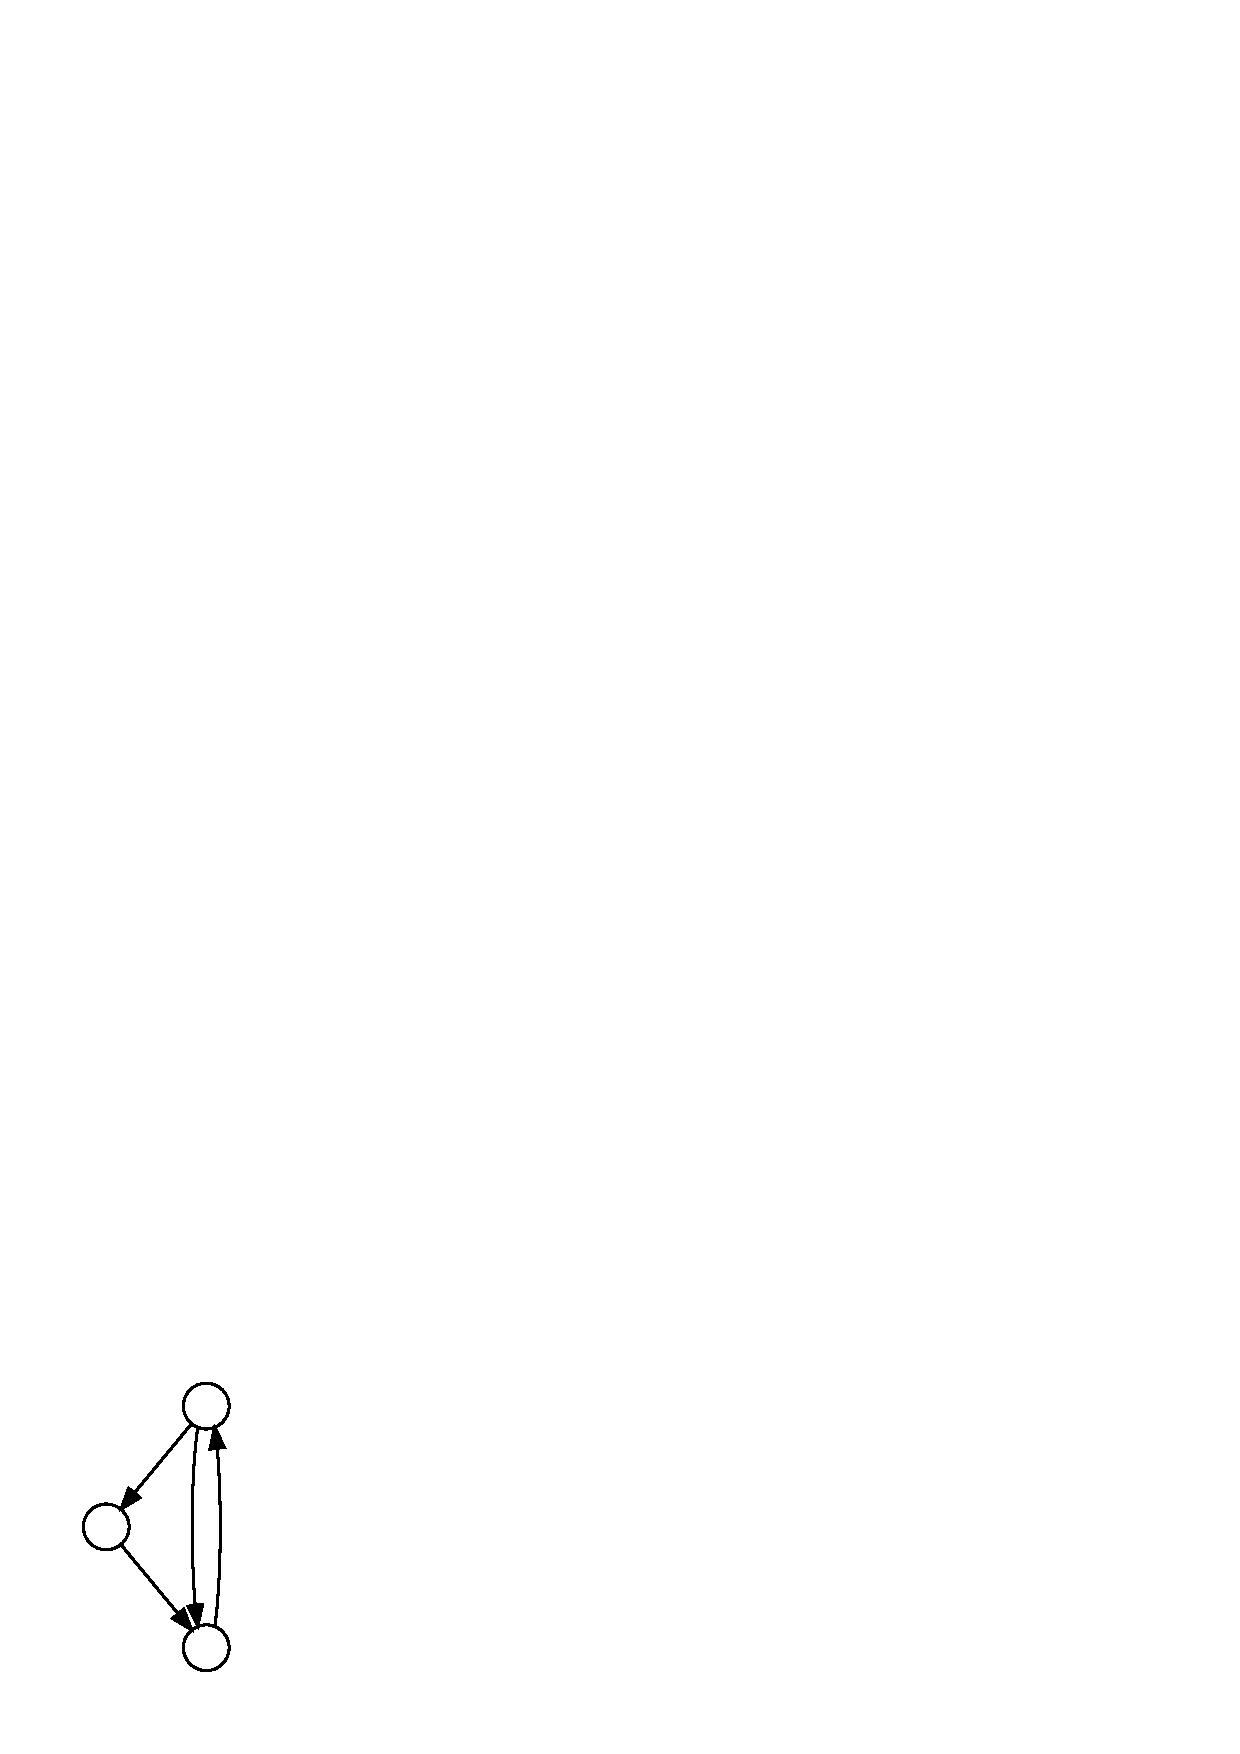
\includegraphics[height=0.03\textheight]{M2-plain} &
    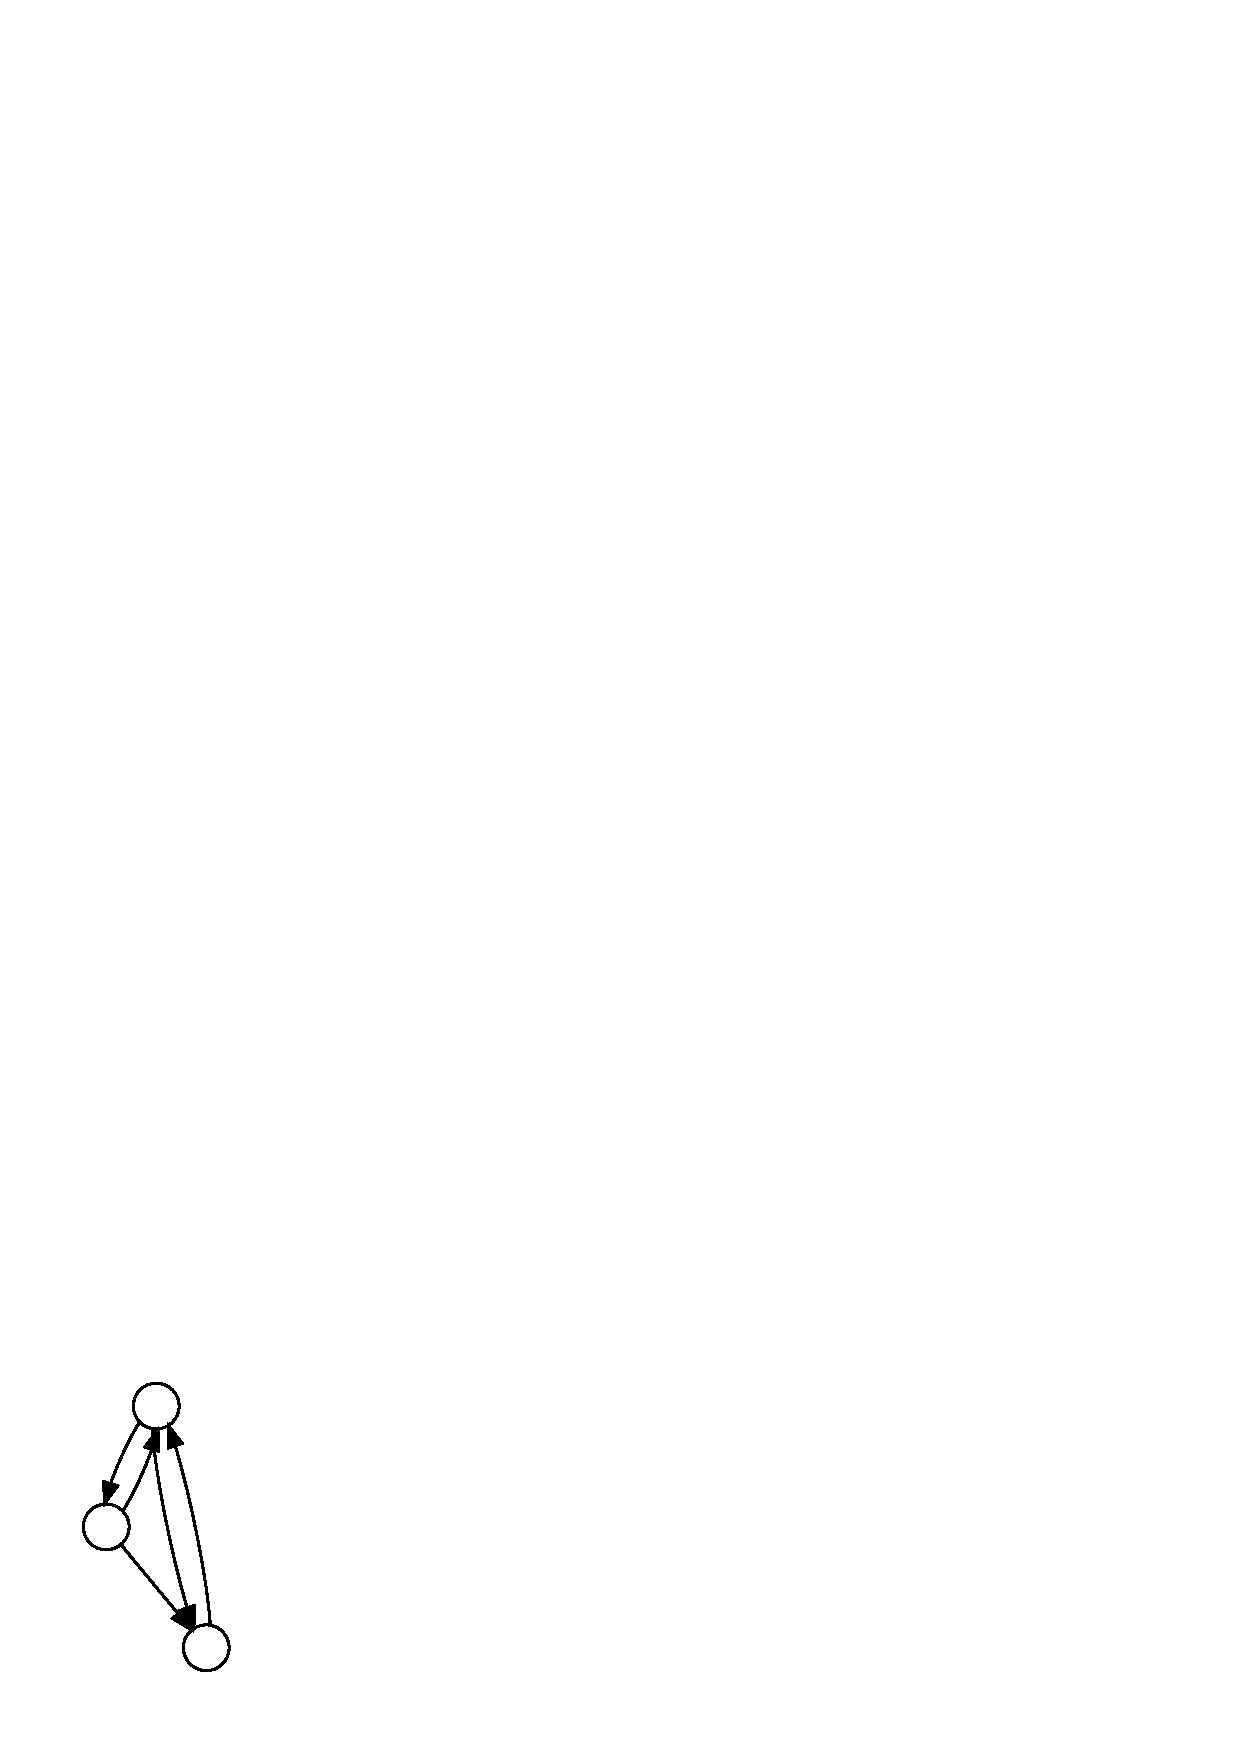
\includegraphics[height=0.03\textheight]{M3-plain} &
    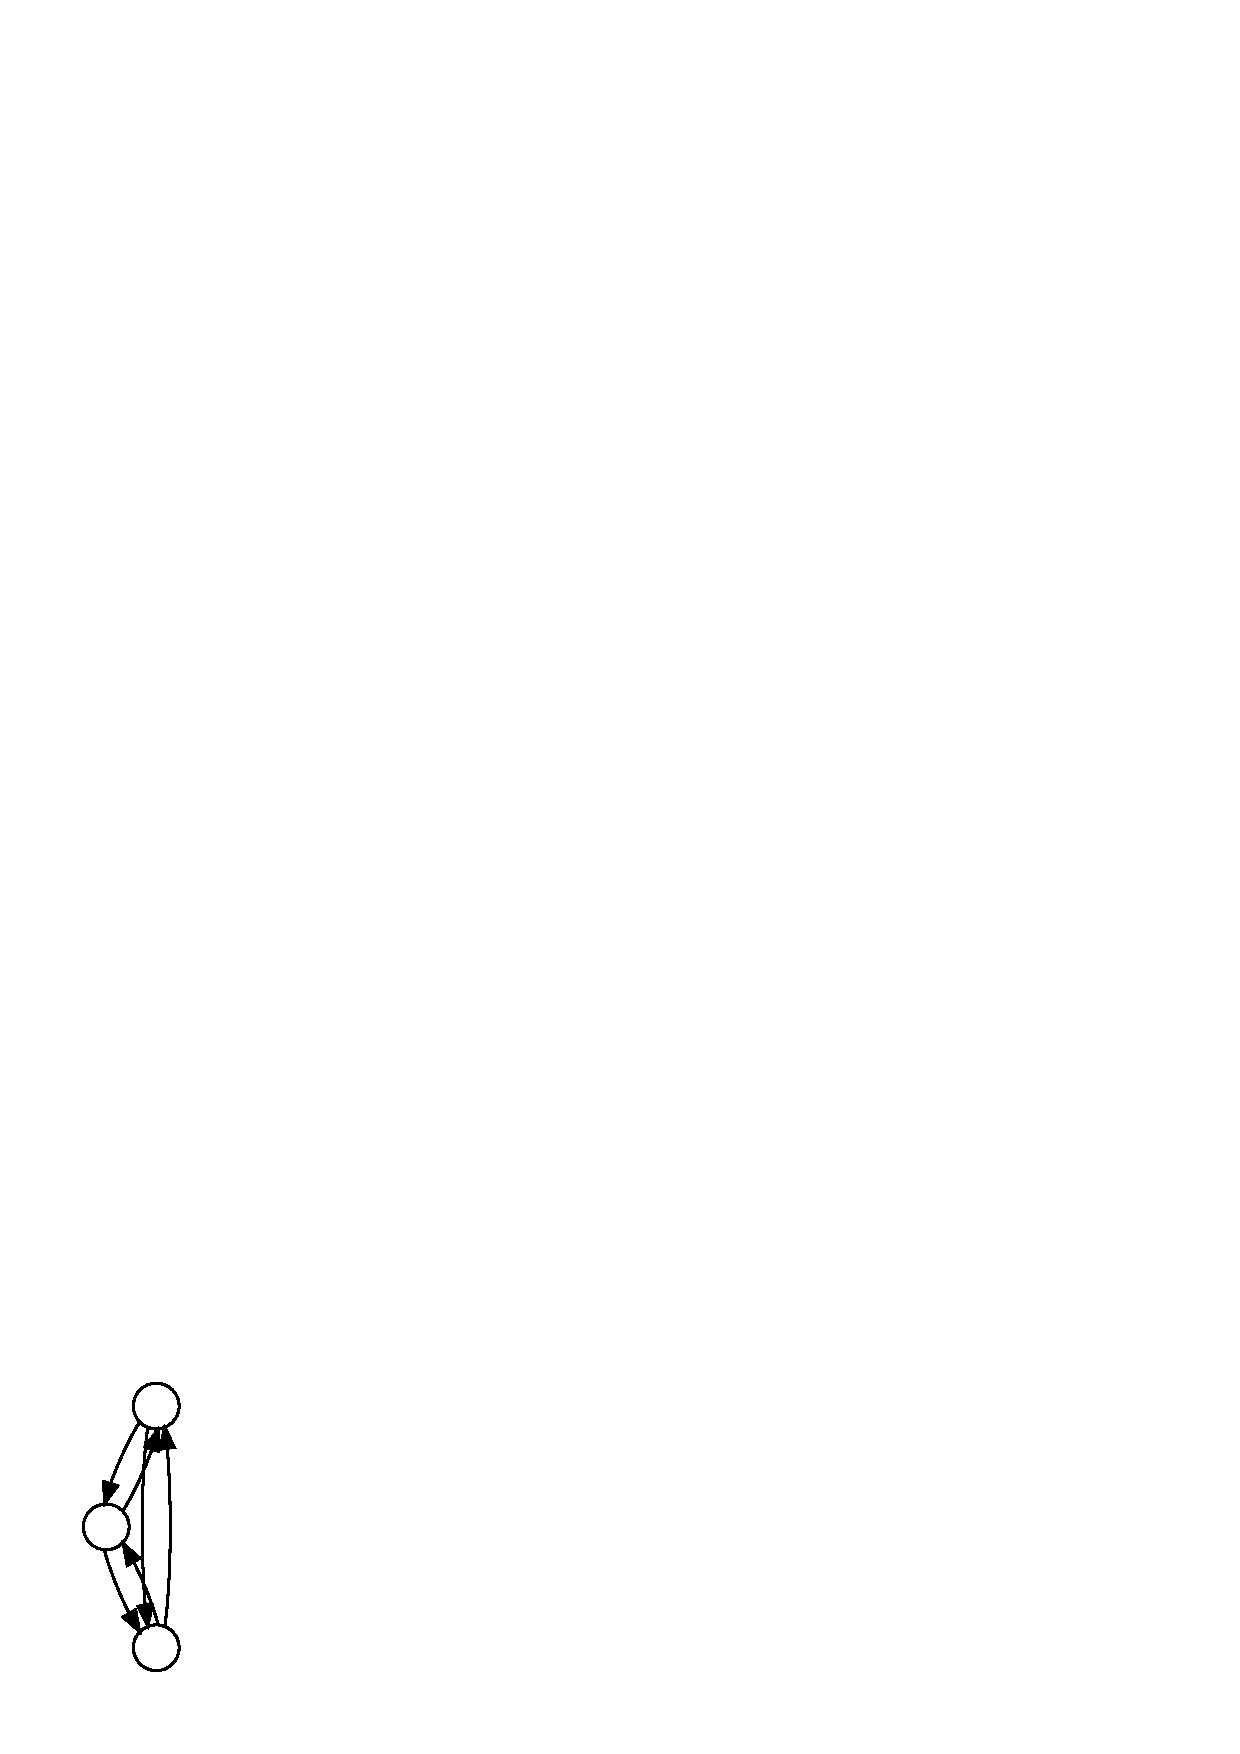
\includegraphics[height=0.03\textheight]{M4-plain} &
    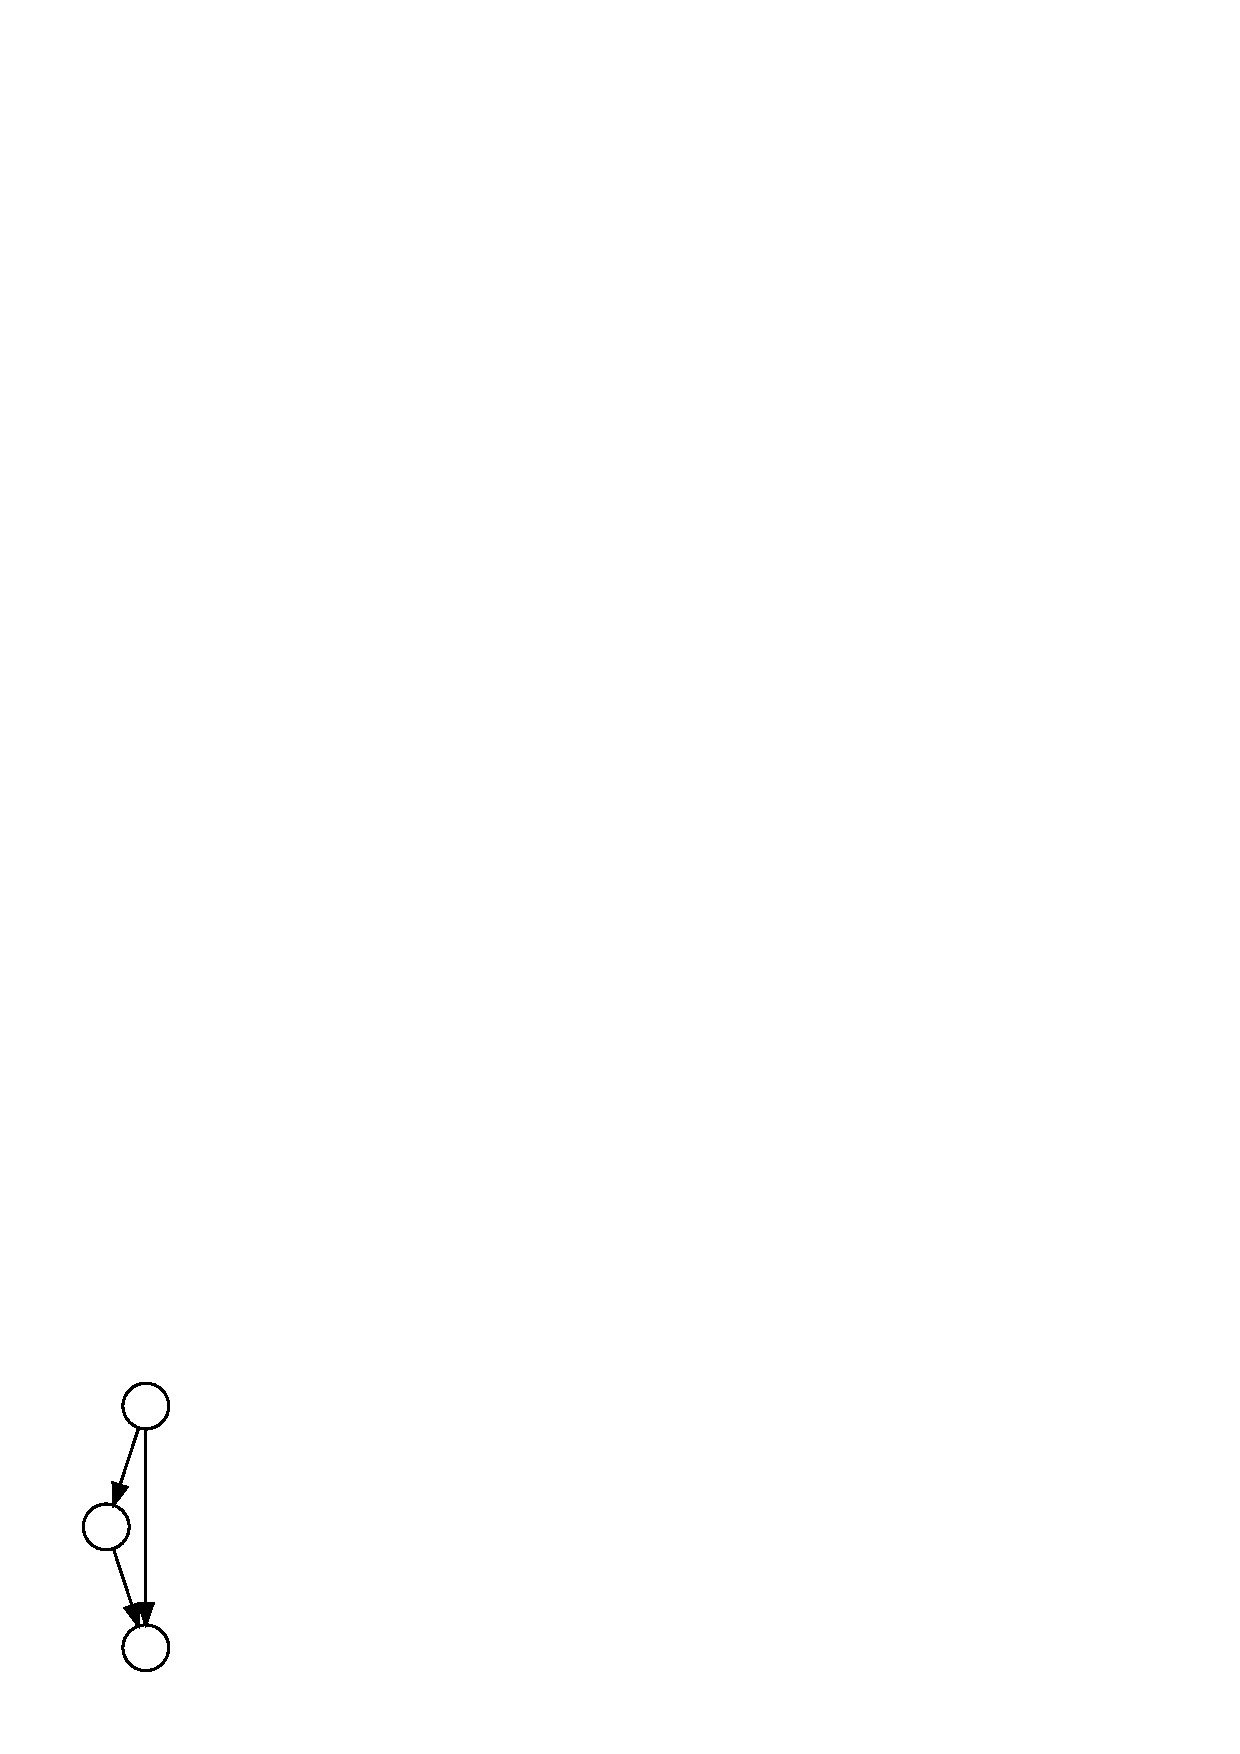
\includegraphics[height=0.03\textheight]{M5-plain} &
    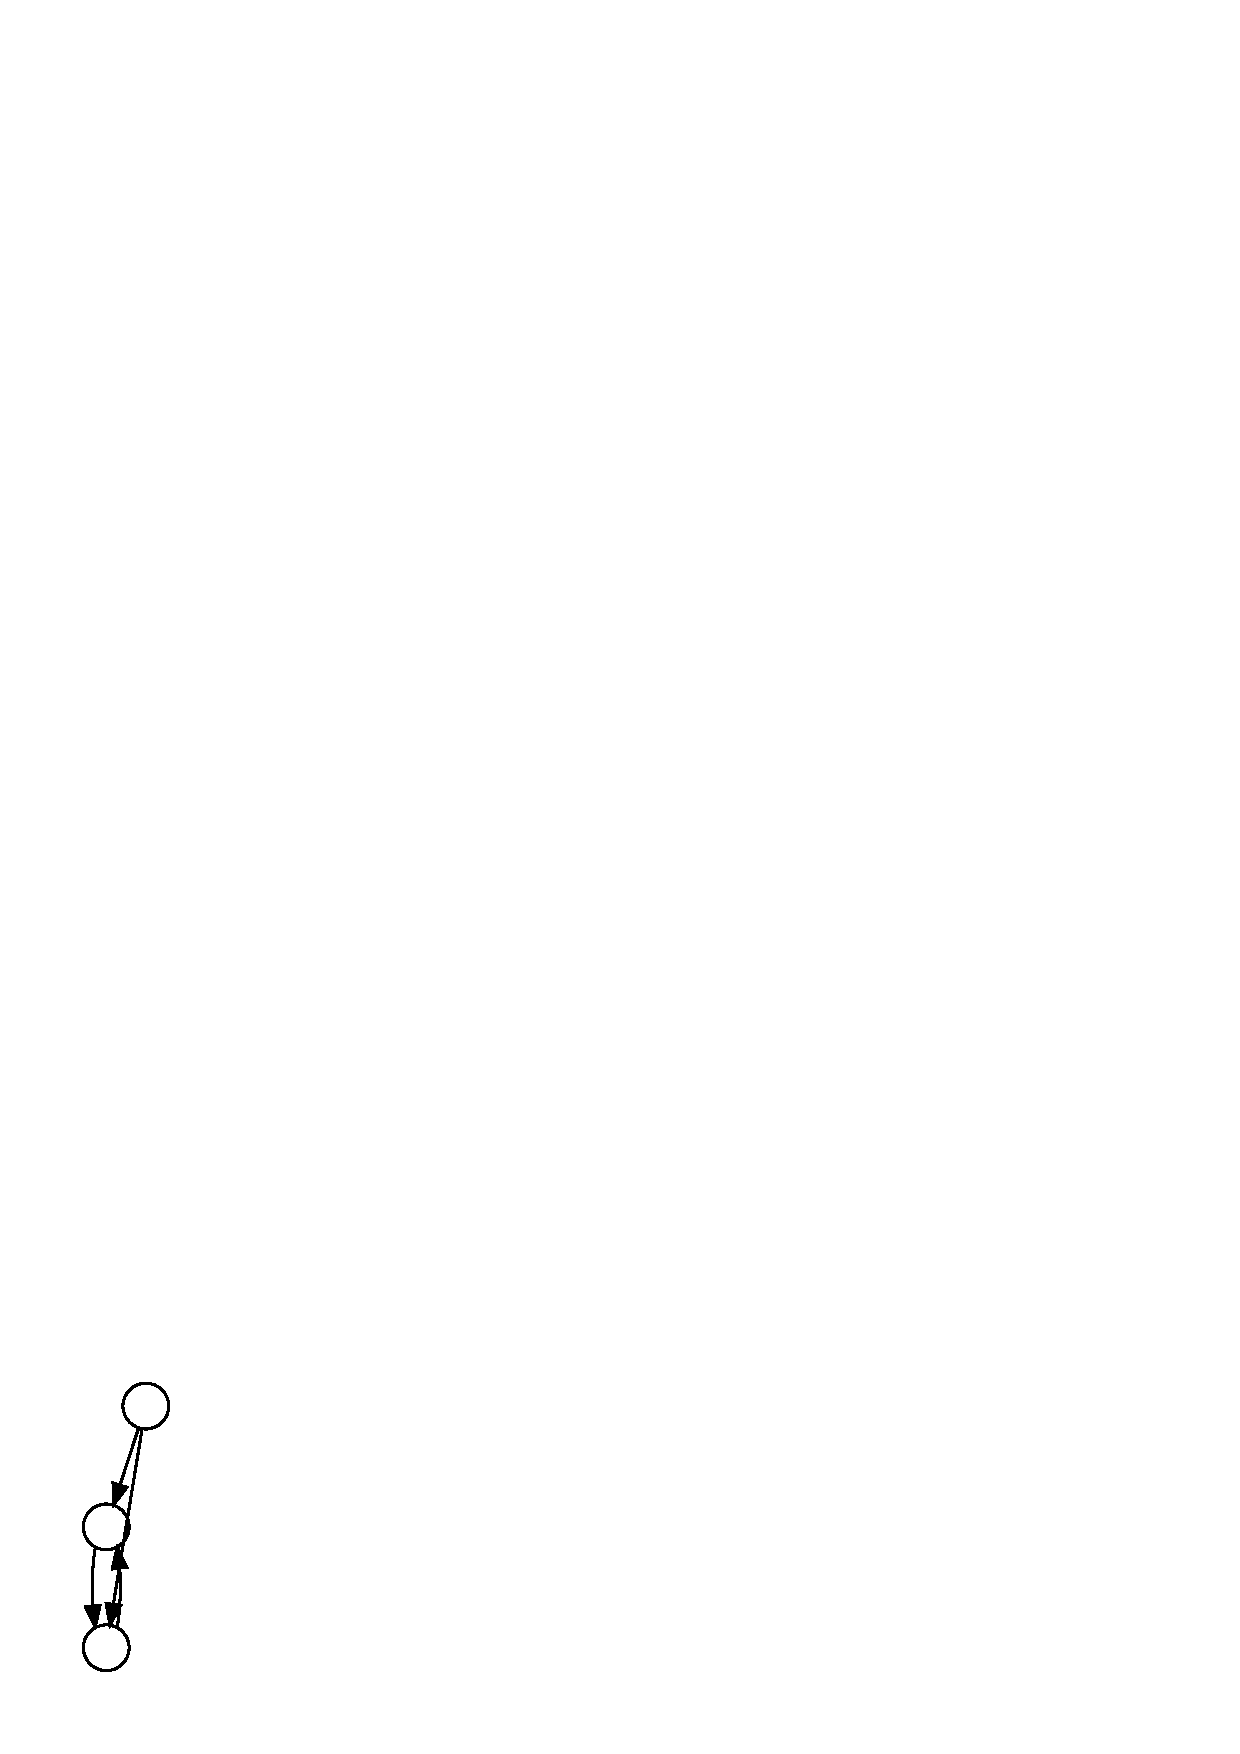
\includegraphics[height=0.03\textheight]{M6-plain} &
    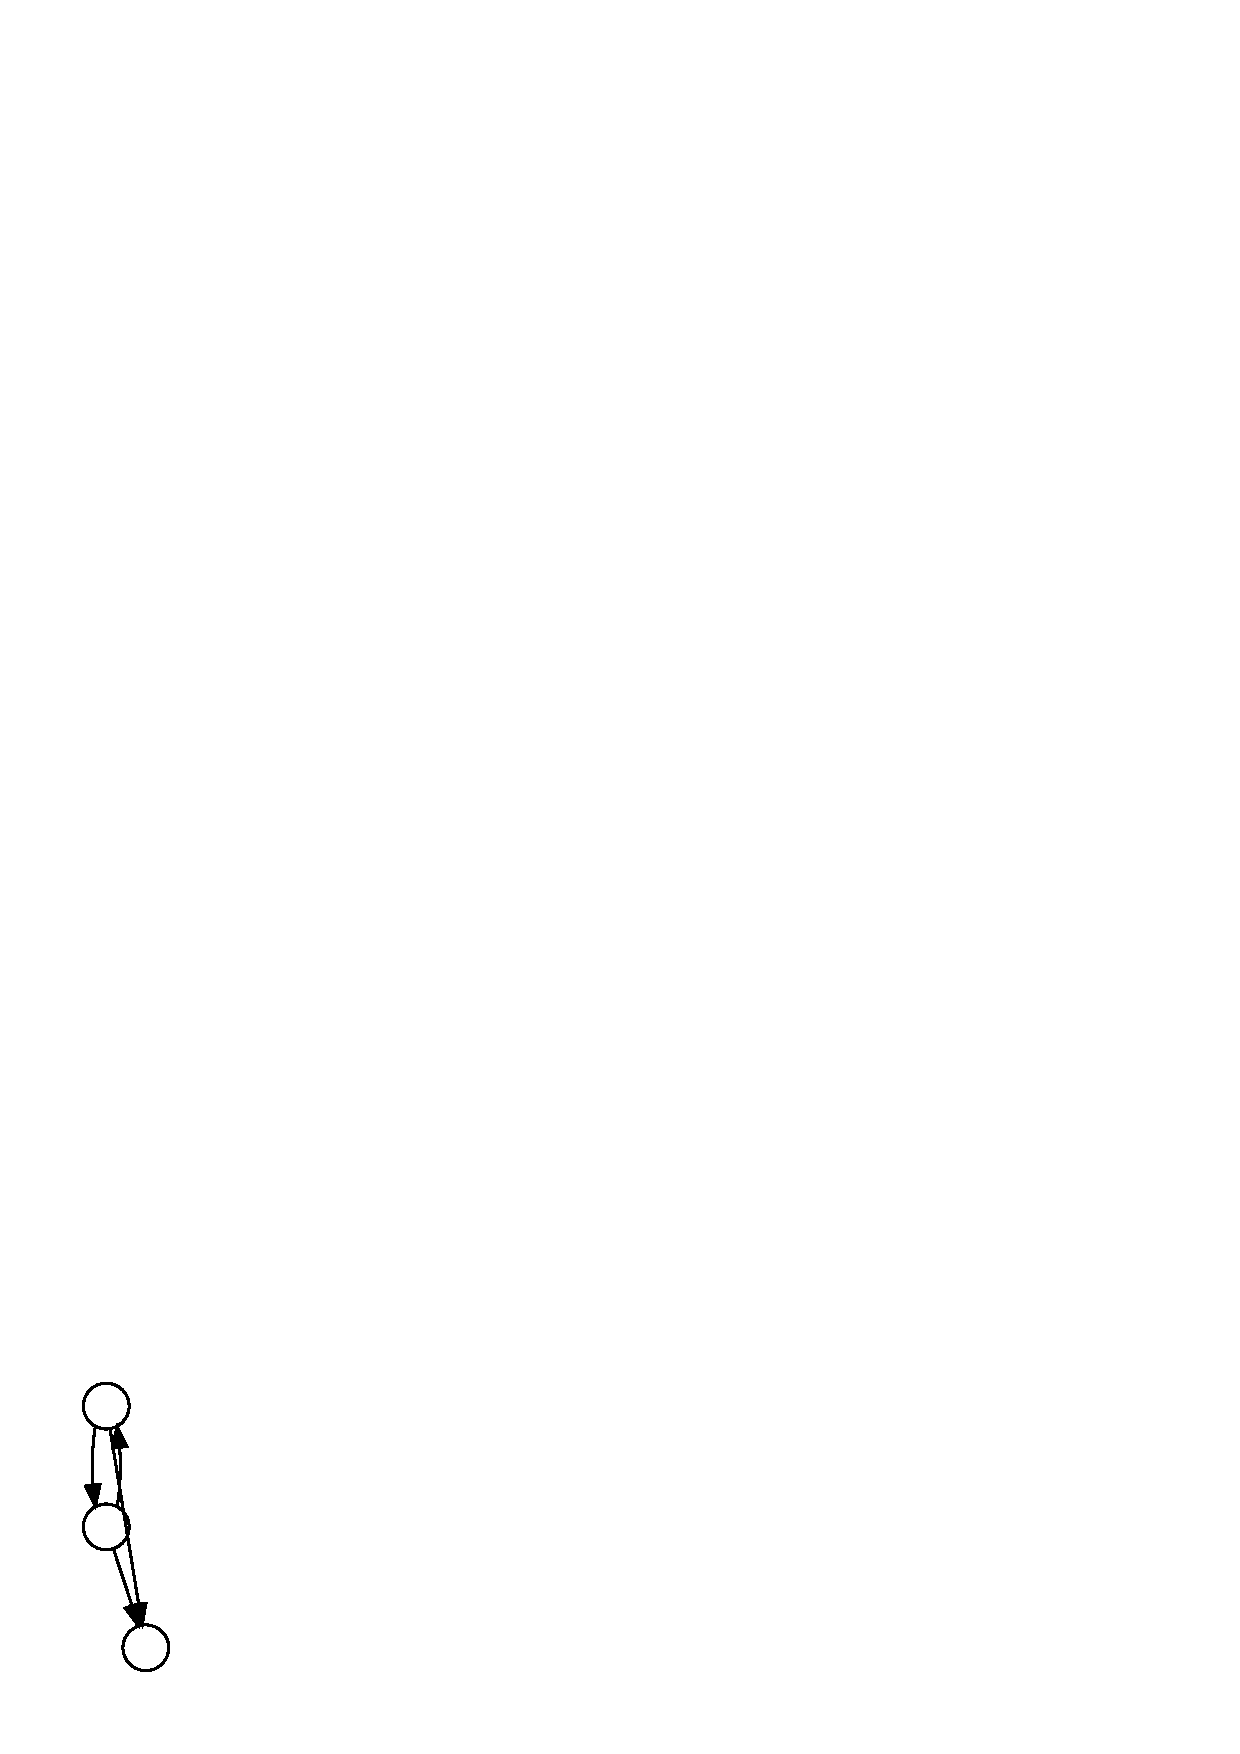
\includegraphics[height=0.03\textheight]{M7-plain} &
    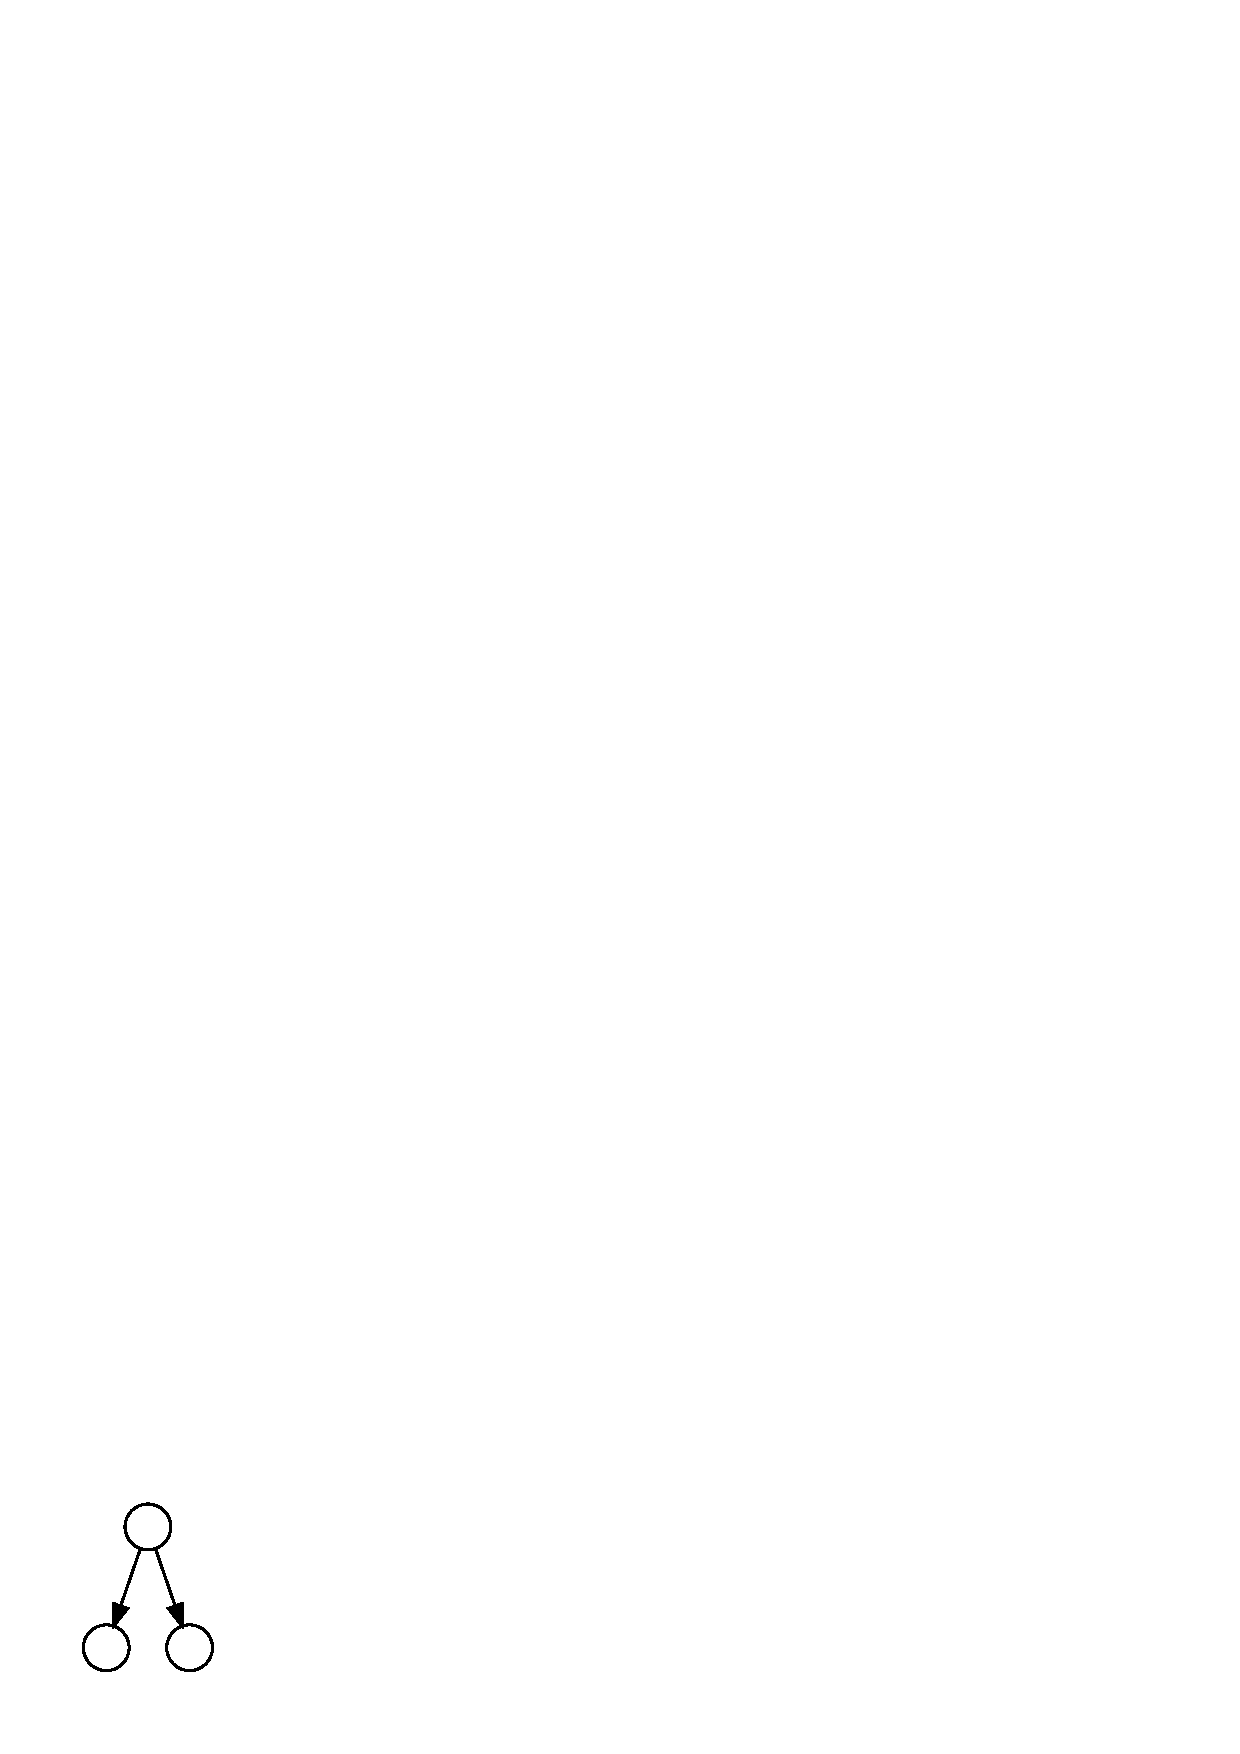
\includegraphics[height=0.03\textheight]{M8-plain} &
    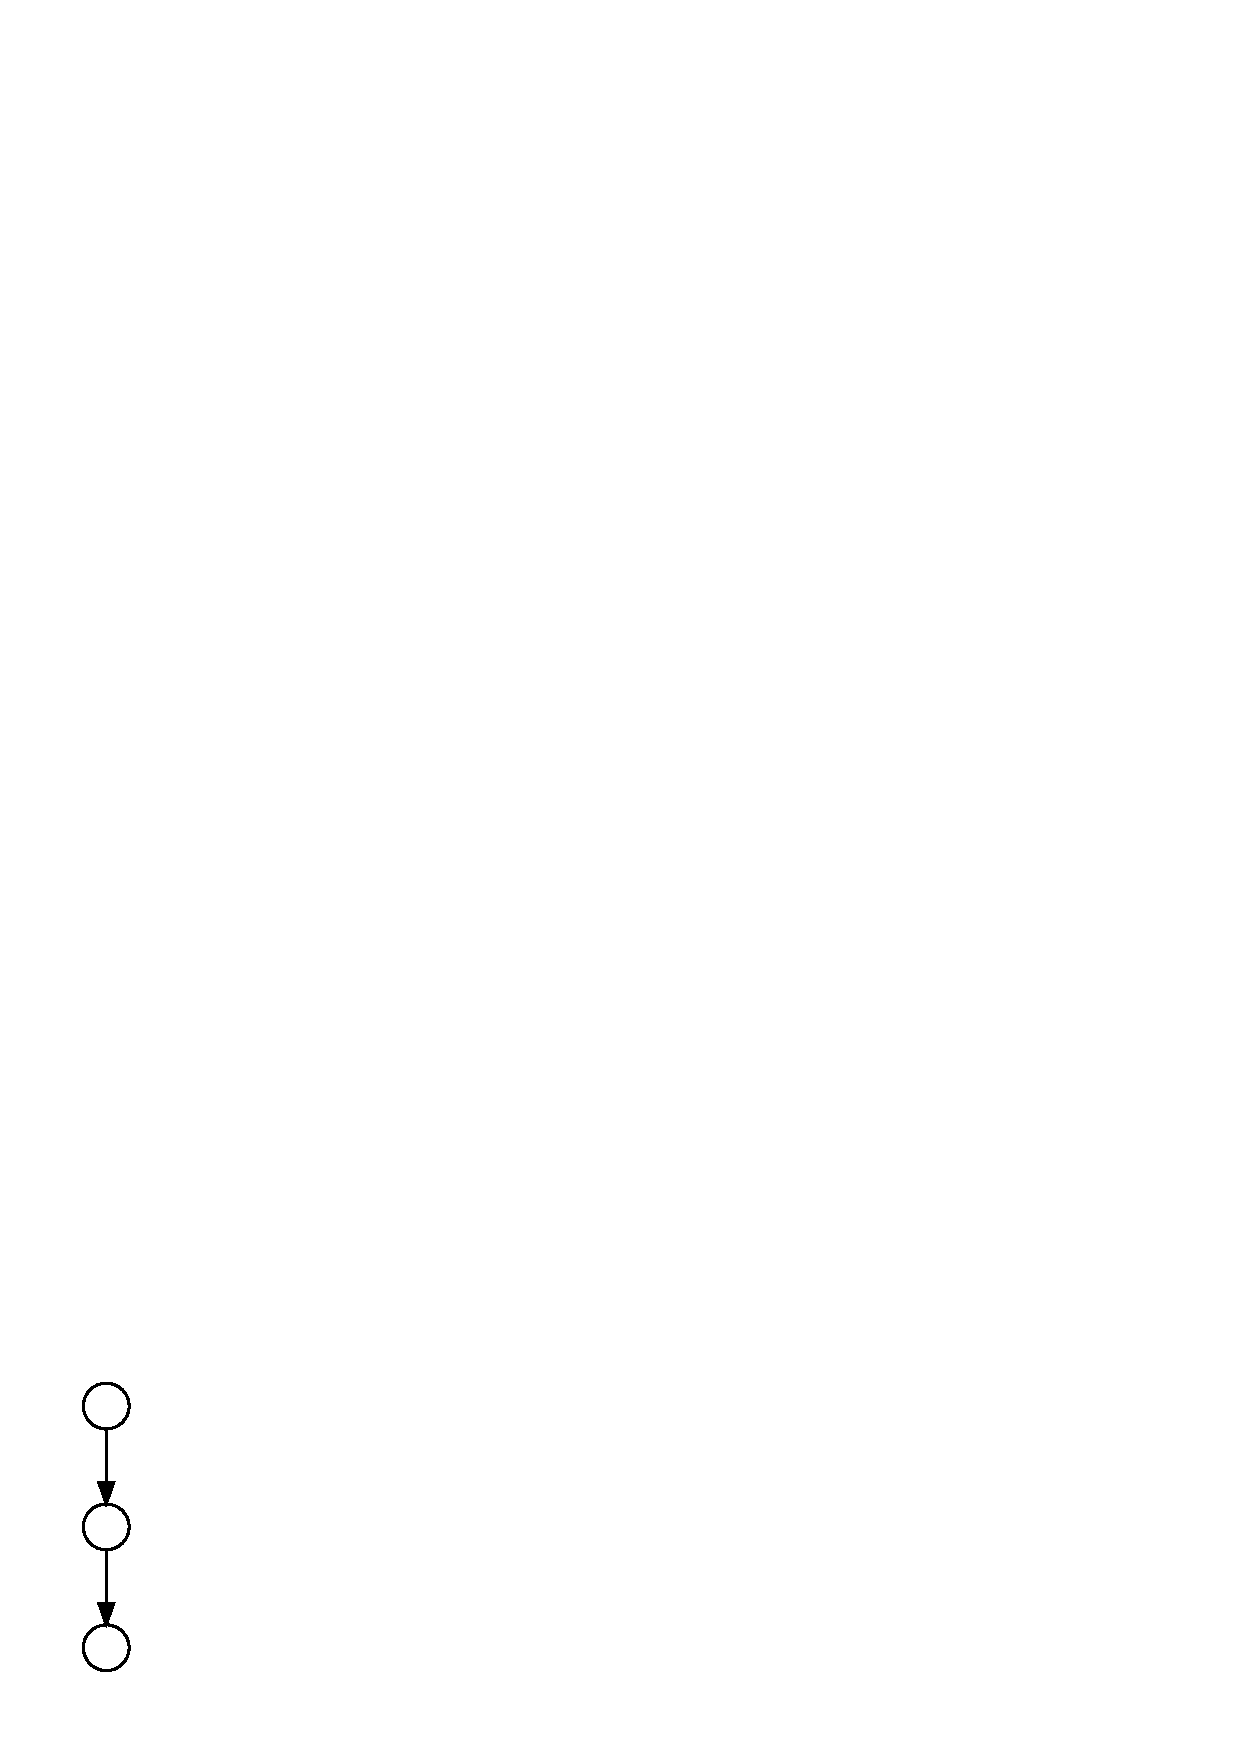
\includegraphics[height=0.03\textheight]{M9-plain} &
    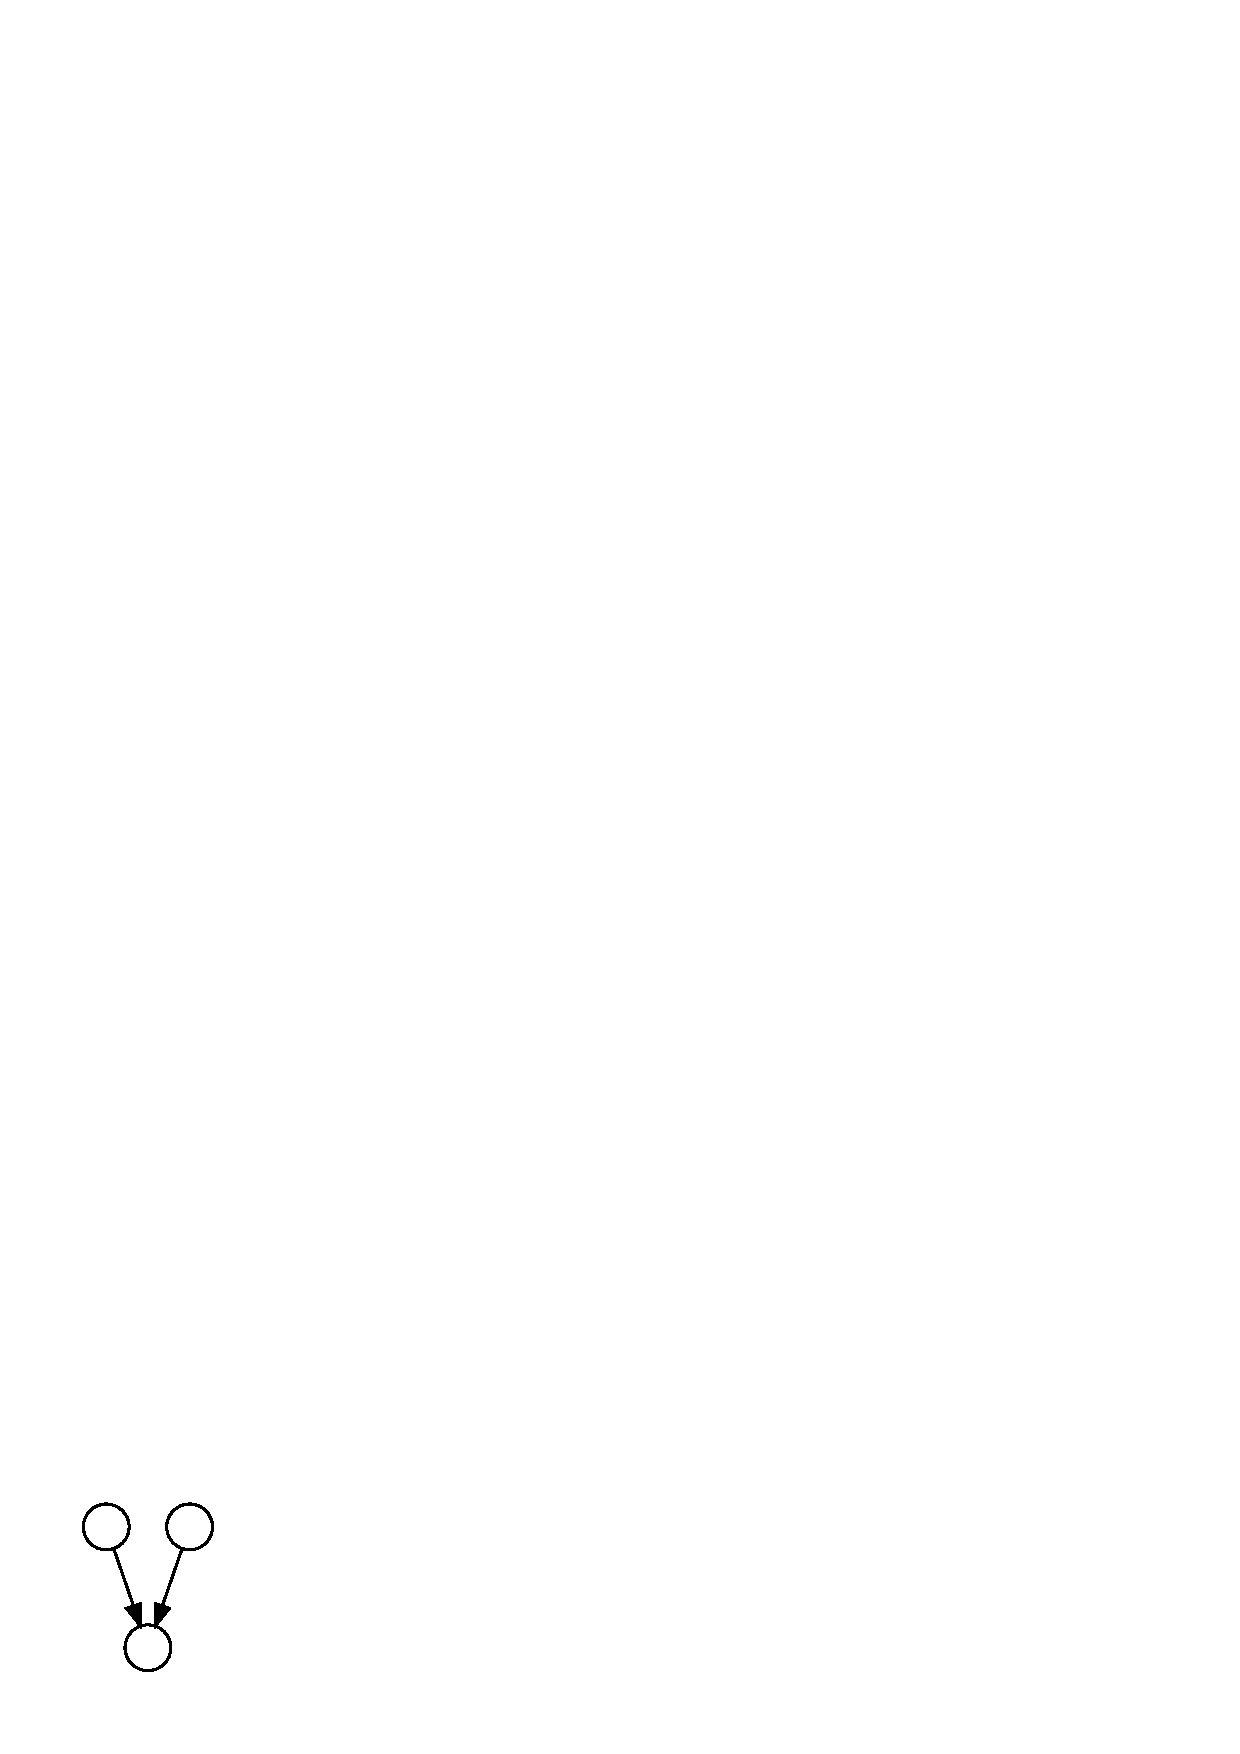
\includegraphics[height=0.03\textheight]{M10-plain} &
    
\includegraphics[height=0.03\textheight]{M11-plain} &
    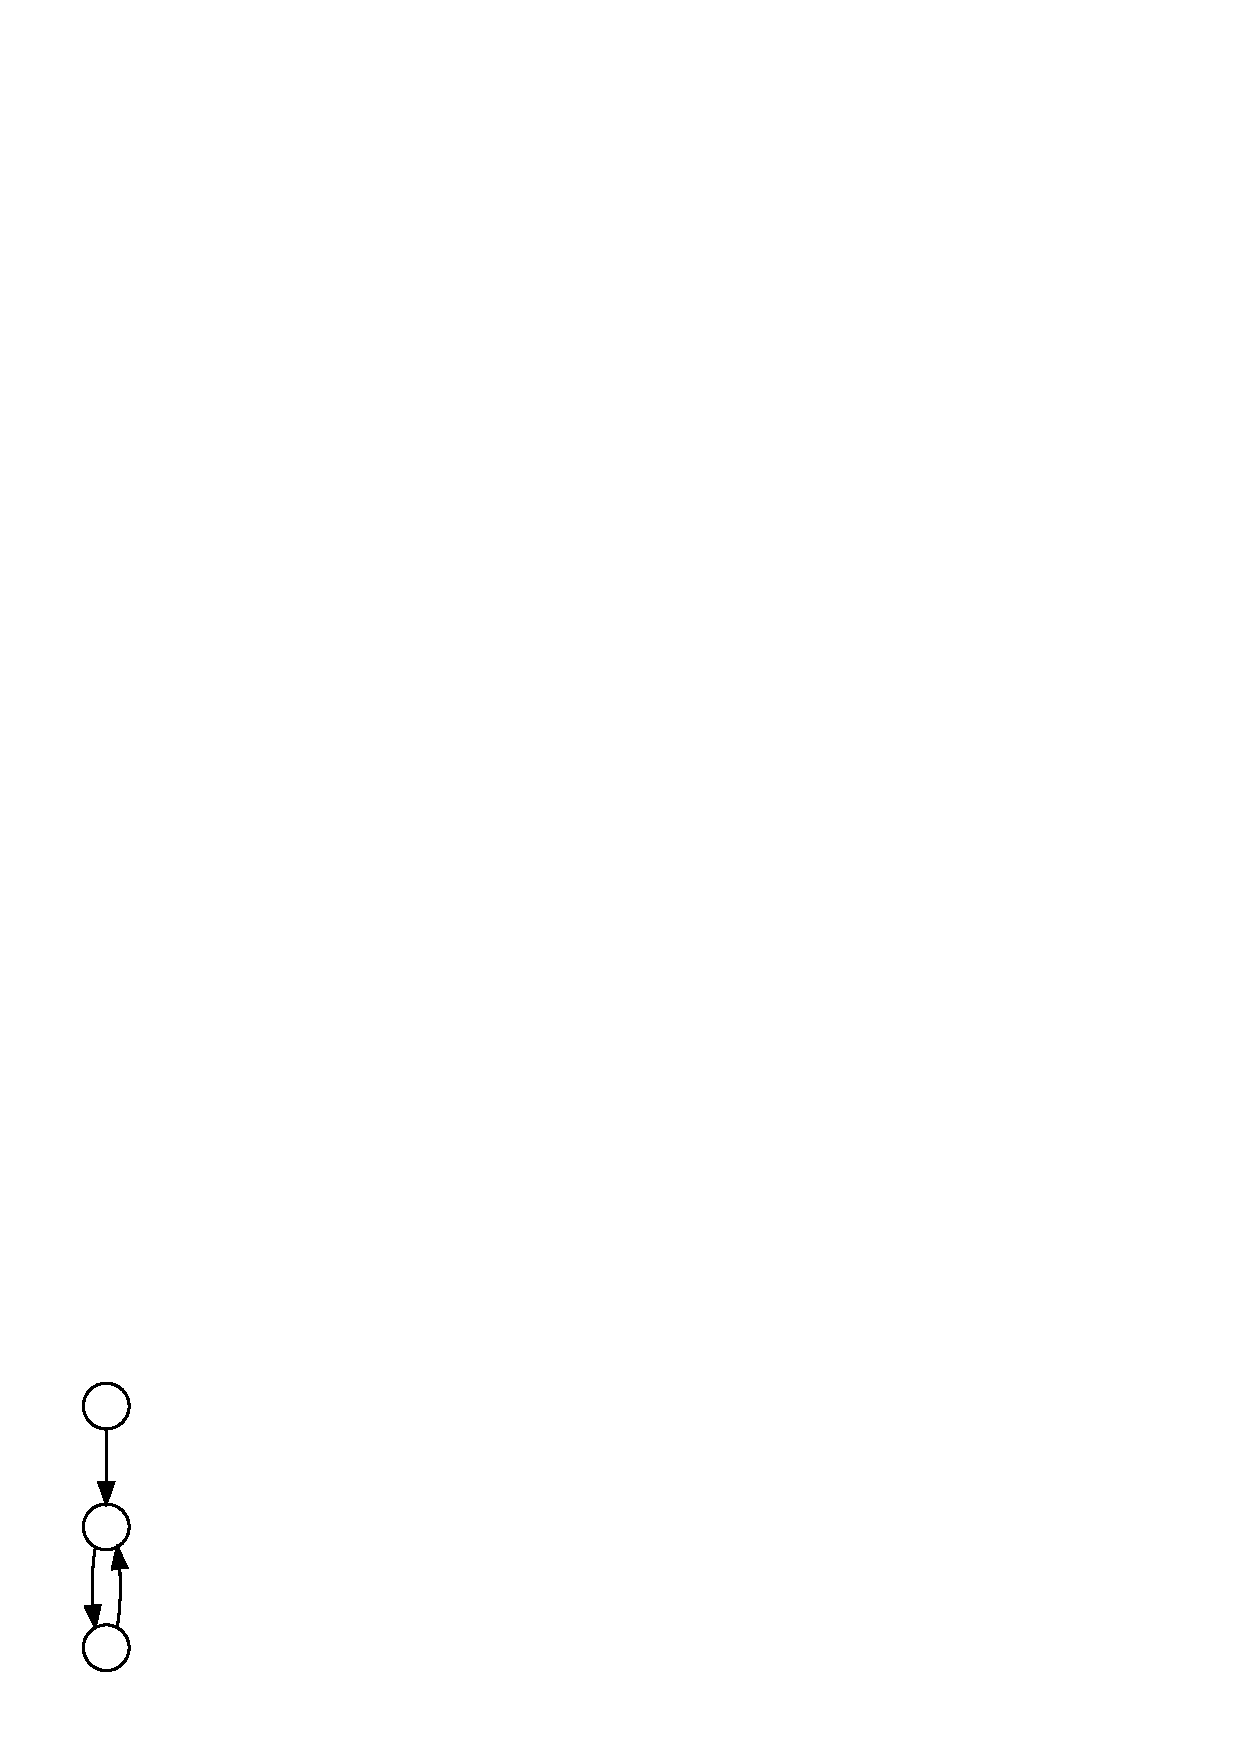
\includegraphics[height=0.03\textheight]{M12-plain} &
    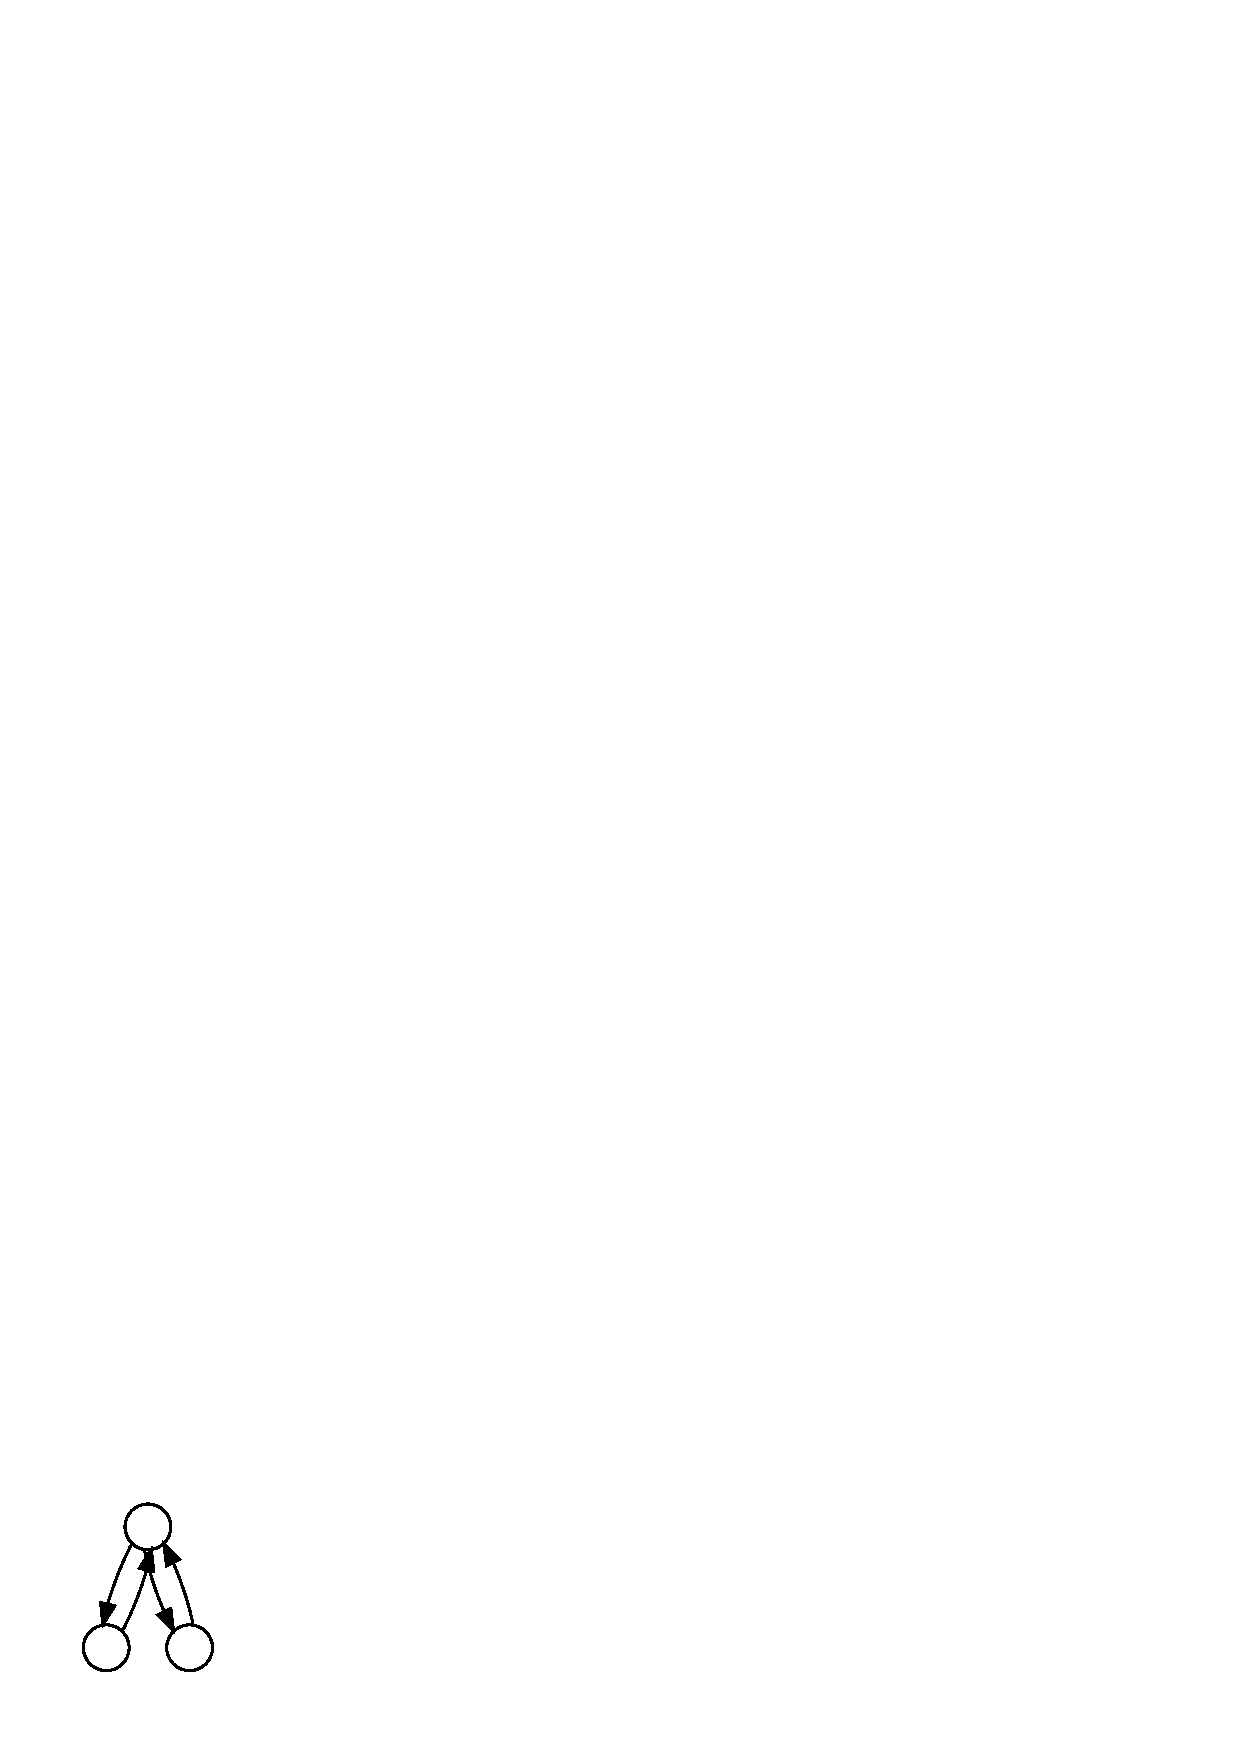
\includegraphics[height=0.03\textheight]{M13-plain} \\
    motif & M1 & M2 & M3 & M4 & M5 & M6 & M7 & M8 & M9 & M10 & M11 & M12 & M13
    \\ \hline
    $Z$ & -379.0 & 496.4 & 6,523 & 1,171,385 & 1,055 & 3,566 & 4,604 & 1,411 &
    -867.2 & 2,599 & 1,293 & 1,387 & 40,286 \\
    NMI & 0.44 & 0.40 & 0.48 & 0.64 & 0.23 & 0.43 & 0.46 & 0.11 & 0.09 & 0.09 &
    0.20 & 0.23 & 0.42
  \end{tabular}
  \caption{Motif significance $Z$ compared to a random network and normalized
    mutual information score for motif clustering using each of the 13 motifs.}
  \label{tab:motifs}
\end{table*}

\begin{table}[t!]
  \centering
  \begin{tabular}{l|ll}
    Algorithm & Louvain Modularity & Clauset-Newman-Moore \\ \hline
    NMI & 0.1 & 0.27
  \end{tabular}
  \caption{The normalized mutual information scores of the other algorithms we
    used.}
  \label{tab:others}
\end{table}

\section{Discussion}

\section{Conclusion}

\section{Authors contributions}
All the authors were involved in the preparation of the manuscript.
All the authors have read and approved the final manuscript.

\bibliographystyle{plain}
\bibliography{biblio}

\end{document}

% TEMPLATES FOR TABLES AND FIGURES

%\begin{table}
%\caption{Please write your table caption here}
%\label{tab:1}       % Give a unique label
%\begin{tabular}{lll}
%\hline\noalign{\smallskip}
%first & second & third  \\
%\noalign{\smallskip}\hline\noalign{\smallskip}
%number & number & number \\
%number & number & number \\
%\noalign{\smallskip}\hline
%\end{tabular}
%% Or use
%\vspace*{5cm}  % with the correct table height
%\end{table}

%% For one-column wide figures use
%\begin{figure}
%% Use the relevant command for your figure-insertion program
%% to insert the figure file.
%% For example, with the option graphics use
%\resizebox{0.75\textwidth}{!}{%
%  
\includegraphics{leer.eps}
%}
%% If not, use
%%\vspace{5cm}       % Give the correct figure height in cm
%\caption{Please write your figure caption here}
%\label{fig:1}       % Give a unique label
%\end{figure}

%% For two-column wide figures use
%\begin{figure*}
%% Use the relevant command for your figure-insertion program
%% to insert the figure file. See example above.
%% If not, use
%\vspace*{5cm}       % Give the correct figure height in cm
%\caption{Please write your figure caption here}
%\label{fig:2}       % Give a unique label
%\end{figure*}
